
\chapter {Introduction}
\label{sec:intro}


In this document we are going to create a template that will show both the format and the possible content of a model Final Project for the Computer Science studies at the University of Almeria. \footnote{\url{https://www.overleaf.com/read/fsjsmpbcpzkh}} \footnote{\url{https://github.com/imaguila/Dissertation-model--UAL.git}}
It will serve as an aid for the completion of academic work which, during university education, constitutes a permanent activity.

The academic work requires precision and conceptual rigor, mastery of information sources and capacity for theoretical argumentation.  It is not a summary of other people's ideas, but a dissertation on a topic, taking as a reference the information that exists on it in various sources. Remember that copying from one is plagiarism, copying from many is research. \cite{malaga}

This template is written in \LaTeX.
The \LaTeX (written LaTeX in plain text) is a text composition system, oriented to the creation of written documents that present a high typographic quality. Due to its characteristics and possibilities, it is used especially intensively in the generation of scientific articles and books that include, among other elements, mathematical expressions. \cite{wiki}

LaTeX consists of a large set of TeX macros intended to facilitate the use of the typesetting language, \LaTeX, created by Donald Knuth. It is widely used for typesetting academic articles, theses and technical books, given the typographical quality of the documents. 

This language presupposes a different work philosophy from that of the usual word processors (known as WYSIWYG, i.e. <<what you see is what you get>>) and is based on instructions. Traditionally, this aspect has been considered a disadvantage (probably the only one). However, LaTeX, unlike WYSIWYG-type word processors, allows the person writing a document to focus exclusively on the content, without having to worry about the details of formatting. In addition to its graphical capabilities to represent equations, complicated formulas, scientific notation and even music, it allows easy structuring of the document (with chapters, sections, notes, bibliography, analytical indexes, etc.), which provides convenience and makes it useful for academic articles and technical books.

For the elaboration of this guide, in addition to the experience of its author, we have used as a reference the rules on Final Degree Works (TFG) and Final Master Works (TFM) of several Universities, including the University of Malaga \cite{malaga} and University of Alicante \cite{alicante}


\chapter{General considerations} 
\label{sec:consideraciones}

The list of considerations can be extensive, but there are some key requirements that must be verified.
The writing has a formal character, so that a humorous discourse cannot be developed, nor can sarcasm and the use of colloquial vocabulary be resorted to.  The language used must be technical, rigorous, analytical and precise. 

Although it includes personal work, the first person singular should not be used: "I..."; the formula to be used in the dissertation is the impersonal: "it is proposed...", "the thesis from which it starts..." (and not "I start from the thesis..."), "the thesis from which it starts..." (and not "I start from the thesis...").  (and not "I start from the thesis...").  Thus, the academic style used is characterized by passive verb forms, pronouns and impersonal constructions and specific vocabulary. On some occasions and due to the deformation of the use of English, the first person plural can be used, although in TFG/TFM it is not recommended, unless specific work carried out in a team is described.

The correct use of language (spelling, expression, punctuation marks) is of vital importance.  If necessary, general or specific dictionaries should be consulted to clarify meanings of terms as well as for the use of synonyms and antonyms. 

The fundamental objective of the writing is to demonstrate one's knowledge of the subject as completely as possible. It is important to answer the premises, questions or research or inquiry questions that have been established as a starting point and that will have to be consistent with the objectives of the work.

Form is as important as substance. The coherence of the format is important, especially in the bibliography. It is beyond the scope of this guide to discuss how to make citations and the different types of bibliographies. The university library offers courses and advice for those who need it. It should be noted that each discipline uses different types of citation standards.


In general terms, the academic work consists of four important parts: the introduction, the development, the conclusions and the bibliographical references. In addition to these four, there is a fifth part related to the annexes (complementary and/or explanatory information), although these will be dealt with in detail in chapter \ref{sec:apartados}.  EIt is important to know that the structure of the report is not the one that is followed sequentially when a person plans to write the document. For example, the introduction, which is the first part of any paper, is the last part to be written.

When a person is faced with this type of work, he/she does not obtain a report "at once" or "all at once". Before arriving at the final text, it must have gone through several drafts and numerous changes and rearrangements.

Since close collaboration between students and tutors of the work is necessary, looking for collaborative editing environments can be a good solution. The best recommendation is  \url{https://www.overleaf.com} which, in addition to numerous templates, offers invaluable help on the language \LaTeX{}, which, although not in-depth, does touch briefly on all the topics.

\chapter{Basic rules} 
\label{sec:funda}

The dissertation report must be presented in UNE A4 format, unless the special characteristics of the work presented do not allow it.

\section {Style, Typography and Layout}

The following typeface families may be used: \url{https://tug.org/FontCatalogue/}, typefaces with excessive decoration are not recommended:

	\begin{center}
	\begin{tabular}{p{2cm}p{7.5cm}c}
		\textbf{tyoe} & \textbf{Font} & \textbf{Width} \\ \hline
         Familia 1 & Arial, Helvética, Tahoma  	\ldots & Variable \\
         Familia 2 & Times New Roman, Palatino  Linotype,  	\ldots & Variable  \\
         Familia 3 & Courier  New,  Miriam Fixed \ldots & Fija\\
         \hline
	\end{tabular}
	\end{center}



\begin{table} 
	\begin{center}
	\begin{tabular}{l c c}
		\textbf{type} & \textbf{font} & \textbf{width} \\ \hline
         Familia 1 & Arial, Helvética, Tahoma  	\ldots & Variable \\
         Familia 2 & Times New Roman, Palatino  Linotype,  	\ldots & Variable  \\
         Familia 3 & Courier  New,  Miriam Fixed \ldots & Fija \\
         \hline
	\end{tabular}
	\end{center}

	\caption{\label{tab:letras}Fonts.}
\end{table}


Family 1 is recommended for the headings of the different sections of the document.

Family 2 is recommended for normal paragraphs.

Family 3 is recommended for writing, for example, portions of code, due to its fixed size where tabular text is necessary and aligns perfectly, as well as any other use of fixed font size text.

The use of the Palatino Linotype typeface in italic is recommended for writing simple formulas, for those that are more complex an equation editor can be used, examples:

$ x^2+y^2=r^2,    a+b=c$

If necessary, an equation environment can be used so that it can be referenced later in the text. The equation \ref{ec:ecuacion} is an example, but it becomes a float like tables and figures. The power of \LaTeX{} for equation editing is beyond the scope of this document, we suggest consulting other sources for more information on its use.

\begin{equation}
\label{ec:ecuacion}
    x_1= \frac{-b+\sqrt{b^2-4*a*c}}{2*a}
\end{equation}




The dimensions of the text area are defined through the \emph{geometry}, \lstinline[language=enparrafo]!geometry!, a latex package which in this case is included in the style \textbf{UAL}, \lstinline[language=enparrafo]!\usepackage{UAL}!.

\section {UAL style}

The style defines the front and back cover according to the recommendations of the school of engineering, see figure \ref{fig:facultad}.

\begin{figure}
	\begin{center}
		
\includegraphics[width = 0.5\textwidth]{facultad.png}
	\end{center}
	\caption{\label{fig:facultad} Schoole Logo }
\end{figure}



The generated style allows you to define a single-sided or double-sided document by selecting the "print" option when including the style package (\lstinline[language=enparrafo]!\usepackage[print]{UAL}!). In this way, you can customize whether to go to the odd page in each section or to the next page.
The watermark is also fixed. Other issues incorporated in the style are the different types of headers and footers required.

An important aspect is the floating latex elements, especially tables and figures. These are the elements that can then be incorporated into the indexes of the document header. In cases where "codes" are used, a list index can also be included, \lstinline[language=enparrafo]!\usepackage{listing}!.

If necessary, you can work with the packages for long tables or with those that allow subfigures to be made.

 \section{Figures and tables}

Figures (or graphs) and tables (tables) that are incorporated should be numbered (Arabic numerals) and have a title, and should always be related to the content presented.  All floating elements should be referenced in the text and should preferably be placed after the first time they are cited in the text.

Graphs, photographs, diagrams, maps, drawings, etc. will be considered as figures. It is important to include the origin of the figure in the label; if it was made by the author, the text "own elaboration" should be included.

Graphs, figures and photos should not be included just to fill in, as they are always too noticeable. Graphics and figures should be referenced in the text, otherwise it is better not to include them in the report.



 \section{Listing}

In the computer science domain, it is common that a dissertation/TFM must include portions of formatted code. Even if they are defined as a special floating element. In \LaTeX{} there are many ways to solve this issue. A style called \lstinline[language=enparrafo]!codigo.sty! has been defined that implements an example. The code files are in a separate folder as are the figures. \footnote{It can be synchronized with code repositories like \url{www.github.com} overleaf is used, but it is necessary to maintain two projects}

\subsection{Verbatim environment}
What in latex is placed inside a verbatim environment is no longer latex code and is represented as it appears. But it usually has interactions with the graphic package tikz. so it is not recommended, it is better to use \lstinline[language=enparrafo]!\lstinline!

\begin{verbatim}
#include <stdio.h>

int main()
{
        printf("hello world");
        return 0;
}
\end{verbatim}

\subsection{Listing package}


You can write the code directly inside an environment and if you do not specify anything the default parameters are used. For details on how to configure this utility it is convenient to review the documentation of the package.

\begin{lstlisting}[caption=Ejemplo ]
#include <stdio.h>

int main()
{
        printf("hello world");
        return 0;
}
}
\end{lstlisting}

Example of inclusion without using a floating object. It will not appear in the index by putting \lstinline[language=enparrafo]!nolol=true!.

\lstinputlisting[firstline=1, firstnumber=1, nolol=true]{holamundo.c}


\lstinputlisting[caption=,language=pseudo, caption=Ejemplo en pseudocodigo]{holamundo.psc}

It is really a very complex package that can be complemented by the use of customized environments, the exhaustive exploitation of which is beyond the scope of this style guide.


\chapter {Buenas prácticas}

This section includes a series of questions or good practices derived from experience, basic rules for the preparation of scientific texts \cite{alba2009}, and basic grammatical rules.



\begin{enumerate}
    \item Be careful with the space between words, use \emph{hyphenation} to cut or not words with hyphens. Although by default the latex  package handles it acceptably well.

\item Punctuation marks (commas, periods, semicolons, colons) as well as closing quotation marks, parentheses and question marks must immediately follow (without spaces) the preceding word and be separated by one space from the following word.  Conversely, the opening quotation marks, parentheses and question marks must be separated by a space from the preceding word and immediately before (without a space) the following word.

\item In lists \lstinline[language=enparrafo]!\begin{itemize}! \lstinline[language=enparrafo]!end{itemize}! o enumerations \lstinline[language=enparrafo]!\begin{enumerate}!  where a verb does not appear, i.e. where a complete sentence does not appear, do not put a period at the end. You only put a period at the last item in the list to end the paragraph.

\item  For the same reason, titles and subtitles should not end with a period. In the captions of figures and tables it is at the discretion of the author and tutor, but the recommendation is not to put it.


\item The first time an acronym is used it must be defined, including the text of the definition in parentheses and capitalizing the letters that give rise to the acronym.  Example: MCU (Multipoint Control Unit).  In subsequent appearances of the acronym, the definition should not be included again.  It is recommended that a detailed list of acronyms and their meaning, in alphabetical order, be attached at the beginning of the project.





\item When mathematical symbols are referenced in the text, they should appear in italics and in the same way as they appear in the equations.




\item Be consistent with the use of verb tenses.  If you describe what you have done in the past tense, you must continue with that tense throughout the memory.  




\item All paragraphs conclude with a period.

\item In the text, if numbers are used, they must be expressed with words if they are less than or equal to twenty and with numbers if they are greater than that value or have decimals.


\item  Evaluative terms (adjectives and adverbs) that are exaggerated or unscientific should be avoided. For example, "remarkably" or "substantially" rather than "spectacularly", "enormously", "overwhelmingly", "drastically" or "phenomenally". When speaking of an engineering result or product, "adequately or very conveniently" is preferable to "perfectly".

\item In a scientific text, it is preferable to use "etc." rather than ellipses ("...") to conclude a long list.



\end{enumerate}




 
 \chapter{Sections to define}
\label{sec:apartados}

As indicated in section \ref{sec:intro}, in addition to the title page and identification data, the reference sections of the work will have four distinct parts (introduction, development, conclusions and bibliographical references) and the annexes.

 \section{Bloque inicial de identificación}

 \subsection{Portada y contraportada}  
La portada es la presentación del trabajo en la que se ha de indicar el título y subtítulo (si  lo  hubiera),  el  autor  o  la  autora  del  mismo,  el  nombre  del  tutor  o  de  la  tutora,  el  Grado  que  cursa, la institución y el año. Su formato está fijado por la ESI.


\paragraph{Titulo}

Debe describir el contenido del trabajo, 10 o 15 palabras. Un buen título nos servirá para identificar el objetivo principal del estudio.

\paragraph{Resumen }
Debe contener:
\begin{itemize}
    \item El  propósito  del  trabajo  en  una  o  dos  frases
    \item El  diseño  y metodología  utilizada
    \item Los  resultados  más  significativos  del trabajo realizado 
    \item Un breve resumen de las conclusiones.
\end{itemize}


 \subsection{Portadilla}
A decisión del autor del trabajo se puede incorporar una dedicatoria, y también una copia del resumen de la contraportada. En el caso de no encuadernarse el trabajo \footnote{se ha seleccionado la opción \emph{print} al incorporar el estilo y \emph{twoside} al seleccionar la clase latex del documento}, es recomendable incorporar el resumen en esta portadilla.

También se puede añadir una  sección  de  agradecimientos  (evidentemente  no  obligatoria)  define  un apartado  donde  el autor  puede  (y  quizás  debe)  referenciar  a  aquellas  personas  y/o  instituciones  que,  de  manera generosa, han colaborado de algún modo en la gestación y desarrollo del TFG/TFM.
Igualmente el autor también  puede  utilizar  este  apartado libremente  para mencionar  a  aquellos  familiares,  compañeros, amigos, etc., de los que ha recibido apoyo personal, moral o afectivo. 

 \subsection{Índices y listas}

Cada índice puede o no  comenzar en una nueva página (utilizando el comando  \lstinline[language=enparrafo]!\clearpage! , se incluirán los índices que se estimen necesarios, en este orden:

\begin{itemize}
    \item Índice de contenidos: (obligatorio  siempre)  se  incluirá  un  índice  de  las secciones  de  las  que  se  componga  el  documento,  la  numeración  de las divisiones  y  subdivisiones  utilizarán  cifras  arábigas y harán mención a la página del documento donde se ubiquen.
    
\item Índice de figuras: si el documento incluye figuras se podrá incluir también un índice con su relación, indicando la página donde se ubiquen.

\item Índice de tablas: en caso de existir en el texto, ídem que el anterior.

\item Índice de listados: en caso de existir en el texto, ídem que el anterior.

\item Índice de abreviaturas, siglas, símbolos,etc.:en  caso  de  ser  necesarios  se podrá incluir cada uno de ellos.

\end{itemize}

 \section{Introducción}
Se hará énfasis a la importancia de la temática, su vigencia y  actualidad;  se  planteará  el  problema  a  investigar,  así  como  el  propósito  o finalidad de la investigación. En cuanto a incluir o no un anticipo de las conclusiones habitualmente depende del tipo de trabajo y suele estar a criterio de tutor.

Cabe destacar la necesidad de incorporar los objetivos si no se utiliza un apartado específico para ello.

 \section{Desarrollo o cuerpo del documento}
Incluye   el  desarrollo  de  los  aspectos  esenciales  del  tema.  Aquí  se  evidenciará la capacidad de organización y estructuración de los argumentos de quien escribe. Se han de evitar las contradicciones y asegurar la coherencia entre las ideas expresadas. El desarrollo se  basa  en  la  exposición,  en  el  análisis  reflexivo  y  en  el  contraste  de  ideas.  En  este  proceso  argumentativo,  las  ideas  principales  y  secundarias  deben  ir  acompañadas  de  \textbf{citas  de  fuentes  bibliográficas} y de ejemplos que lograrán sustentar la tesis principal del trabajo. 
%%%%%%%%%%%%%%%%%%%%%%%%%%%%%%%%

Los objetivos del trabajo o bien se han definido en la introducción o se describen como primer apartado del cuerpo del documento.

En informática en la Universidad de Almería (UAL) si bien todos los trabajos son monográficos, también cierto que la mayor parte de ellos tienen una componente puramente técnica de desarrollo de aplicaciones software, donde se aplica alguna metodología de desarrollo de software \cite{SWEBOK2014}. El apartado desarrollo deberá balancear la componente  técnica con la de investigación propia de un trabajo monográfico.

En el aspecto mas investigador,  es  importante  destacar  dos  aspectos \cite{alicante}:  
\begin{itemize}
    \item [Primera]  Es  muy  importante  la  relectura  de  las  fuentes. No basta con   resumir   lo  leído  sino  que hay que   analizarlo. % hay  que  procurar  contrastar  la  información  recogida  con  la  perspectiva  personal.  
    \item [Segunda]   Nunca  se  debe  tomar  como  propias  las  ideas  de  otras  personas;  esto  es  plagio  académico. Toda  información  recabada    debe  ser  especificada  como  tal,  es  decir,  debe  ser  citada la fuente de la que procede.
    
\end{itemize}


Si el TFG involucra el desarrollo de software de aplicación es en este apartado donde se debe indicar el proceso y / o metodología seguida. Se describirán todas las etapas del desarrollo, así como las herramientas utilizadas. Pero la memoria no se puede convertir en una lista de artefactos del proceso software. Los anexos son una buena oportunidad para mostrar el trabajo realizado sin enmarañar la memoria.



 \section{Conclusiones}
Obligatoriamente se incluirá una sección de conclusiones donde se realizará  un  resumen  de los objetivos  conseguidos  así  como de  los resultados obtenidos si proceden.
\begin{itemize}
\item Deben ser breves y responder específicamente a los objetivos
planteadas en su caso en  la Introducción o en el apartado objetivos.
\item  Las recomendaciones que se formulen han de ser viables y
deben sugerir, además, en qué línea hay que seguir investigando como trabajo futuro.
\item Discutir las implicaciones de los resultados para la práctica  del campo de la informática.

\end{itemize}



 \section{Bibliografía}
  Se  incluirá    la  relación  de  obras  y  materiales consultados  y  empleados  en  la  elaboración  de  la  memoria  del  TFG.
   Podrá  utilizarse  cualquier  sistema bibliográfico normalizado    predominante    en    la    rama    de conocimiento, se debe acordar con el tutor.

 \section{Anexos}
Se incluirán tantos como sea necesario. Se recomienda incorporar los artefactos generados en el desarrollo del proyecto software como anexos para agilizar la lectura de la memoria. Se debe recordar que la memoria del TFG no es un documento técnico sino académico.



 
 \chapter {Apartado de INTRODUCCIÓN}


En lo que atañe al contenido de esta sección \ref{sec:intro}, como cualquier introducción es importante que se cumpla con la norma de ser breve y recoger tanto el problema como el enfoque de la solución planteada en el trabajo fin de grado.

Se hará una introducción al ámbito del trabajo, comenzando por el contexto general y aproximándose progresivamente a los aspectos más concretos que se traten. Es conveniente  terminar  con  una  exposición  clara  de  los  objetivos.

Los objetivos si bien se incluirán en la introducción pueden aparecer al inicio del cuerpo del trabajo con su propio subapartado.

Debe responder a las siguientes preguntas:
\begin{itemize}
    \item ¿Qué se sabe del tema que se quiere investigar?
    \item ¿Para qué se quiere estudiar ese tema concreto?
    \item ¿Qué  se  quiere  saber  sobre  ese  tema  concreto?  (hipótesis, preguntas, objetivos de investigación) En  este  apartado  se  deben  ir  insertando  referencias  bibliográficas pertinentes.
\end{itemize}

Otras pequeñas consideraciones sobre este apartado son:
\begin{enumerate}
    \item  \textbf{Contextualiza al lector}. La introducción cumple el rol de sumergir al lector en el contexto en el que se  centra el resto de la memoria.
    \item  \textit{Constituye la primera impresión}. Es importante que dedicar un tiempo considerable a escribirla porque será la primera impresión que los lectores tendrán sobre el trabajo realizado. La introducción a un trabajo debe incorporar la hipótesis y los principales argumentos, aunque intentando que sea, a la vez, concisa, breve, creativa y analítica.

\item \underline{ Sirve para centrarse}. La introducción de un trabajo lleva al lector de lo general a lo particular. Lo importante es que, si bien se puede optar por una primera frase general, esta debe contextualizar, pero no tiene que estar demasiado alejada del tema principal. Se ha de pisar el suelo.

\item \textsc{Actúa como “gancho”}.  Se puede comenzar con un ejemplo, con una cita de texto interesante, una anécdota inesperada o una pregunta disparadora, pero sin pasarse.
    
\end{enumerate}


Pero  tal como se dice en la figura \ref{fig:recintro}, es lo último a escribir en la redacción del  trabajo fin de grado.


\begin{figure}
	\begin{center}
		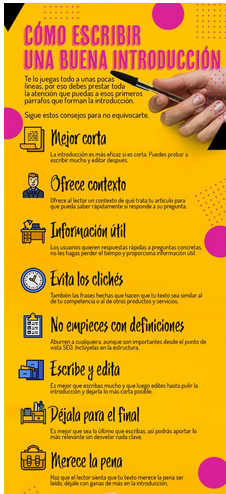
\includegraphics[scale = 0.95]{Figures/intro.png}
	\end{center}
	\caption{\label{fig:recintro} Recomendaciones sobre la introducción}
\end{figure}



